\documentclass[a4paper, 10pt]{article}
\usepackage[utf8]{inputenc}
\usepackage[danish]{babel}
\usepackage{verbatim}
\usepackage{amsmath}
\usepackage{listings}
\usepackage{graphicx}

\title{Fundations of Computer Graphics\\ Ugeopgave 2}
\author{Mads Ohm Larsen}

\begin{document}
\maketitle

\section{Introduktion}
Vi skal i denne uge redegøre for vores \textit{LineRasterizer}.
En lineraterizer er et objekt, som kan finde ud af hvor på skærmen vores linier skal tegnes.
I denne opgave forsøger vi ikke at skabe dybde eller at interpolere henover hverken farve eller dybde.
Det betyder at vores implementation i slutningen af denne rapport kun er i stand til at tegne linier på skærmen og ikke i rummet.
Det betyder også at vi ikke giver vores linie world coordinates, men derimod blot hvor på skærmen de skal begynde og slutte.

\section{Linier}
%%%%%%%%%%%%%%%%%%%%%
% HVAD ER EN LINIE? %
%%%%%%%%%%%%%%%%%%%%%
\subsection{Hvad er en linie?}
Allerførst skal vi kigge på hvad en linie rent faktisk er og hvordan vi forstår udtrykket at tegne en linie.
En linie kender vi fra de allerførste matematiktimer vi havde tilbage i folkeskolen.
Udtrykket ligger os derfor ikke fjernt, og vi har alle en god forståelse for hvad en linie er.
I folkeskolen lærte vi at en lige linie altid er givet ved:

\begin{equation}
y = ax + b \label{ll}
\end{equation}

Dette har vi siden fundet ud af at dette ikke var helt sandt.
Tager vi f.eks. og tegner en lige linie, som er lodret, kan vi ikke beskrive ligning (\ref{ll}).
Det ville ellers have været nemt at bruge ligning (\ref{ll}) til at tegne lige linier på skærmen.
Man ville kunne gøre dette som følger

\lstset{language=C, basicstyle=\footnotesize, numbers=left, stepnumber=2, numberstyle=\tiny, frameround=tttt, frame=tlBR, captionpos=b}
\begin{lstlisting}
void drawline( int x0, int y0, int x1, int y1 )
{
    int x;
    double y    = y0;
    double step = ( y1 - y0 ) / ( x1 - x0 );

    for( x = 0; x <= x1; x++ ) {
        drawdot( x, Round(y) );
        y += step;
    }
}
\end{lstlisting}

Her finder vi hældningen mellem start- og slutpunktet og bruger dette til at tælle \texttt{y} op.
Dette er både forkert (mht. lodrette linier) og langsomt, da vi bruger for meget tid på at rode rundt med flydende tal, som alligevel bliver rundet af, så de passer til pixel positioner.

Vi skal altså bruge en bedre måde at repræsentere vores linie på.
Vi har heldigvis en anden parameterfremstilling for en lige linie, nemlig den homogene ligning for en lige linie.
Denne er givet ved

\begin{equation}
l:\ \Big\lbrace \left( x, y \right) | \left( a, b \right) \cdot \left( x - x_0, y - y_0 \right) = 0 \Big\rbrace
\end{equation}

Denne kan hurtigt skrives om til

\begin{align}
\left( a, b \right) \cdot \left( x - x_0, y - y_0 \right) &= 0 \nonumber\\
a \left( x - x_0 \right) + b \left( y - y_0 \right) &= 0 \nonumber\\
ax + by - \left( ax_0 + by_0 \right) &= 0 \nonumber\\
l:\ \Big\lbrace \left( x, y \right) | ax + by + c = 0 \Big\rbrace \nonumber
\end{align}

hvor $-\left( ax_0 + by_0 \right) = c$.

Dette betyder at $l: ax + by + c = 0$ er liningen for en lige linie.
Her har vi altså at den afhænger af hældningen, skæring med y-aksen og et start punkt (et hvilket som helst punkt på linien).

%%%%%%%%%%%%%%%%%%%%%%
% HVOR LANGT ER DER? %
%%%%%%%%%%%%%%%%%%%%%%
\subsection{Hvor langt er der?}
Når vi skal til at tegne pixels, skal vi finde ud af hvilken side af linien der er tættest på en pixel, og altså hvilken pixel der skal "tændes".
Det betyder at vi skal bruge afstanden fra et punkt til linien.
Afstanden mellem en linie og et punkt, er enhedsnormalen til linien prikket med forskellen mellem et punkt på linien og det punkt vi vil finde afstanden til.
Sagt med andre ord, hvis $(a, b)$ er vores normal, $(x_0, y_0)$ ligger på linien og vi vil finde afstanden til $(x,y)$ har vi følgende formel:

\begin{equation}
d(x,y) = \frac{(a,b)}{\sqrt{a^2 + b^2}} \cdot (x-x_0, y-y_0) \label{afstand}
\end{equation}

Afstanden er positiv, hvis vi er på samme side som normalvektoren og negativ ellers.
Dette kan vi bruge til at finde ud af hvilken af to pixels, som skal tændes, om det er den over eller under linien.

Regner vi lidt på (\ref{afstand}) får vi 

\begin{align}
d(x,y) &= \frac{(a,b)}{\sqrt{a^2 + b^2}} \cdot (x-x_0, y-y_0) \nonumber\\
       &= \frac{a(x - x_0) + b(y - y_0)}{\sqrt{a^2 + b^2}} \nonumber\\
       &= \frac{ax + by + c}{\sqrt{a^2 + b^2}} \nonumber
\end{align}

Vi har allerede sagt at hvis punktet ligger over linien er denne positiv, under er den negativ og hvis den er på linien er afstanden nul.
Vi behøver derfor ikke at regne $\sqrt{a^2 + b^2}$ da $ax + by +c$ vil have samme nulpunkter som (\ref{afstand}).
Vi har nu

\begin{equation}
F(x,y) = ax + by + c = d(x,y) \sqrt{a^2 + b^2} \label{normafstand}
\end{equation}

som også vil have den egenskab at være positiv hvis vores punkt ligger på samme side som normalen, nul hvis den ligger på linien og negativ, hvis punktet på modsatte side af normalen.

%%%%%%%%%%%%%%%%%%%%%%%
% HVOR NORMAL ER DEN? %
%%%%%%%%%%%%%%%%%%%%%%%
\subsection{Hvor normal er den?}
Vi skal nu have fundet vores normal.
Hvis vi starter med at antage at hældningen $|\alpha|$ er mindre eller lig med nul, og vi kender start- og slutpunkt på ligningen er hældingen $|\alpha|$ givet ved

\begin{equation}
|\alpha| = |\frac{dy}{dx}| \leq 1 \nonumber
\end{equation}

, hvor $dy = y_{stop} - y_{start}$ og $dx = x_{stop} - x_{start}$.

En lige linie kan nu udtrykkes som

\begin{equation}
y = \alpha x + \beta = \frac{dy}{dx}x + \beta \nonumber
\end{equation}

Hvilket er ekvivalent med 

\begin{equation}
ax + by + c = (dy)x - (dx)y + (dx)\beta = 0 \nonumber
\end{equation}

Vores normal vektor $(a,b)$ er altså lig med $(dy, -dx)$ når hældningen $|\alpha| \leq 1$
Heldigvis er vores linier lige, og vi kan derfor blot spejle dem når vi skal tegne linier med hældning større end 1. 
Dette betyder, for vores normal, at vi blot bytter om på $dy$ og $dx$, samt alle andre forekomster af $x$ og $y$.

%%%%%%%%%%%%%%%%%%%%%%%
% LAD OS TEGNE PIXELS %
%%%%%%%%%%%%%%%%%%%%%%%
\subsection{Lad os tegne pixels}
Hvis vi antager at vi netop har tegnet en pixel i punktet $(x_p, y_p)$ og skal til at tegne det næste, hvordan gør vi så dette?
Jo, vi vil gerne tegne den pixel der ligger tættest på linien.
Vi skal altså se hvilken en af $(x_p + 1, y_p)$ og $(x_p + 1, y_p + 1)$ som ligger tættest på vores linie.
Dette ville være dobbelt arbejde at finde ud af, da vi jo allerede ved, fra (\ref{normafstand}) at $F(x,y)$ er positiv hvis vi ligger på samme side som normalen, negativ på den anden side og nul hvis vi ligger på linien.
Vi kan altså blot indsætte "midterpunktet"\footnote{Denne pixel eksistere selvfølgelig ikke, da vi kun har heltal} i denne ligning, altså finde ud af om 

\begin{equation}
d_p = F(x_p + 1, y_p + \frac{1}{2}) = a(x_p + 1) + b(y_p + \frac{1}{2}) + c \label{dp}
\end{equation}

 er større eller mindre end $0$.
Antager vi at denne er kendt, og at vi gerne vil finde den næste i rækken, er denne givet ved 

\begin{align}
d_{p+1} &= F(x_p + 2, y_p + \frac{3}{2}) \nonumber\\
        &= a(x_p + 2) + b(y_p + \frac{3}{2}) + c \nonumber\\
        &= a(x_p + 1) + b(y_p + \frac{1}{2}) + c + a + b
\end{align}

, hvis vi vælger den øverste af de to pixels, eller

\begin{align}
d_{p+1} &= F(x_p + 2, y_p + \frac{1}{2}) \nonumber\\
        &= a(x_p + 2) + b(y_p + \frac{1}{2}) + c \nonumber\\
        &= a(x_p + 1) + b(y_p + \frac{1}{2}) + c + a
\end{align}

, hvis vi vælger den nederste.
I begge ligninger er første del lig med (\ref{dp}) og den eneste forskel er det sidste led, som vi vil kalde $\Delta NE$ henholdsvis $\Delta E$.
Disse er altså lig med $a + b$ henholdsvis $a$.
Det betyder at for at finde det næste punkt hvor vi skal tegne en pixel, skal vi blot bruge det punkt vi har og så lægge $\Delta NE$ til hvis det næste punkt skal være over linien eller $\Delta E$ hvis det skal være under.

%%%%%%%%%%%%%%
% Algoritmen %
%%%%%%%%%%%%%%
\subsection{Algoritmen}
Vi vælger til at starte med et startpunkt $(x_{start}, y_{start})$.
Dette punkt vil være på den linie vi skal til at tegne, derfor 

\begin{equation}
ax_{start} + by_{start} + c = 0 \nonumber
\end{equation}

i følge (\ref{ll}).
Vi har derfor at

\begin{align}
d_0 &= F\left( x_{start} + 1, y_{start} + \frac{1}{2} \right) \nonumber\\
    &= a(x_{start} + 1) + b(y_{start} + \frac{1}{2}) + c \nonumber\\
    &= ax_{start} + by_{start} + c + a + \frac{1}{2}b \nonumber\\
    &= a + \frac{1}{2}b \label{zero}
\end{align}

Men hov, nu har vi jo gået så meget igennem for at komme af med alle decimal tallene og nu ender vi med at vores decisionvariabel afhænger af $\frac{1}{2}$.
Vi kan heldigvis gange (\ref{zero}), $\Delta NE$ og $\Delta E$ med 2 og derved stadig beholde nulpunkterne og vi har nu fuldstændig udeladt andet end heltal.

Vi skal nu have implementeret vores algoritme i frameworket.
Her skal vi implementere et par af de funktioner der er givet en skal til.
Det drejer sig om funktionerne \texttt{x()}, \texttt{y()}, \texttt{init( 4 x vector )}, \texttt{more\_fragments()} og \texttt{next\_fragment()}.
De to første funktioner er trivielle, da disse bare skal give x- henholdsvis y-koordinater på den aktive position.
\texttt{init} derimod er lidt mere spændende.
Denne sørger for at initialisere alle de variable vi skal bruge.
Dette har jeg gjort på følgende måde i filen \texttt{line\_rasterizer.h}.

\begin{lstlisting}
void init( vector3_type const& in_vertex1,
	   vector3_type const& in_color1,
	   vector3_type const& in_vertex2,
	   vector3_type const& in_color2)
{
    // This is a line rasterizer
    // The vertices are in 3D screen coordinates
    this->x_start   = in_vertex1[1];
    this->y_start   = in_vertex1[2];
    
    this->x_stop    = in_vertex2[1];
    this->y_stop    = in_vertex2[2];

    this->x_current = this->x_start;
    this->y_current = this->y_start;

    this->dx	    = this->x_stop - this->x_start;
    this->dy	    = this->y_stop - this->y_start;

    this->abs_2dx   = std::abs( this->dx ) << 1; // 2 * |dx|
    this->abs_2dy   = std::abs( this->dy ) << 1; // 2 * |dy|

    this->x_step    = ( this->dx < 0 ) ? -1 : 1;
    this->y_step    = ( this->dy < 0 ) ? -1 : 1;

    this->color_start = in_color1;
    this->color_stop  = in_color2;

    [Choose either x-dominant or y-dominant loop]
}
\end{lstlisting}

Der er intet hokuspokus her, udover linie 20 og 21, hvor vi ganger med $2$ ved at bitshifte en gang til venstre.
Det at loopet skal være x- eller y-dominant er et spørgsmål om hældningen er over eller under $1$.
Som beskrevet tidligere er forskellen blot at bytte om på alle forekomster af x med y og omvendt.
Alt dette har vi gjort således

\lstset{firstnumber=29}
\begin{lstlisting}
// Determine if the line is x-dominat or y-dominant
if ( this->abs_2dx > this->abs_2dy )
{
    // The line is x-dominant
    this->left_right = ( this->x_step > 0 );
    this->d          = this->abs_2dy - ( this->abs_2dx >> 1 );
    this->valid      = ( this->x_start != this->x_stop );

    this->innerloop = &MyLineRasterizer::x_dominant_innerloop;
}
else {
    // The line is y-dominant
    this->left_right = ( this->y_step > 0 );
    this->d          = this->abs_2dx - ( this->abs_2dy >> 1 );
    this->valid      = ( this->y_start != this->y_stop );

    this->innerloop = &MyLineRasterizer::y_dominant_innerloop;
}
\end{lstlisting}

Her deler vi med $2$ ved at bitshifte til højre.
Det andet som er lidt specielt her er at vi sætter \texttt{innerloop} til at pege på en metode, som alt efter om vi er x- eller y-dominant udregner linien rigtigt.

Denne \texttt{innerloop} metode fungere ved simpelthen at regne $d_{p+1}$ ud og derved sætte $(x,y)$-koordinat for den næste pixel, som skal tændes.
Dette bliver gjort for x-dominans som følger

\lstset{firstnumber=1}
\begin{lstlisting}
void x_dominant_innerloop()
{
    if ( this->x_current == this->x_stop ) {
	this->valid = false;
    } else {
	if ( ( this->d > 0 ) 
           || ( ( this->d == 0 )  && this->left_right ) ) {
	    this->y_current += this->y_step;
	    this->d         -= this->abs_2dx;
	}
	this->x_current += this->x_step;
	this->d         += this->abs_2dy;
    }
}
\end{lstlisting}

For y-dominans er det selvfølgelig bare omvendt.

De to sidste metoder vi skulle lave, var \texttt{more\_fragments()} og \texttt{next\_fragment()}.
Disse to er meget simple, da deres opgaver faktisk er meget simple.
Den første returnere blot om der er flere fragments, ved at returnere \texttt{valid}, som kun bliver sat til \texttt{false} når vi er færdige med at tegne linien.

Den anden skal blot steppe en gang frem i vores algoritme, altså skal den blot kalde \texttt{x\_dominant\_loop()} eller \texttt{y\_dominant\_loop()} alt afhængig af hvilken vi er.
Men denne har vi jo sat til at være \texttt{innerloop()}, så vi skal altså blot kalde \texttt{innerloop()} metoden.

\subsection{Hvordan ser det ud?}
Vi har nu fået forklaret og implementeret vores algoritme.
I \texttt{main.cpp} er der lavet to funktioner, som tegner linier.
Disse kaldes ved at køre frameworket og trykke enten \texttt{l} eller \texttt{L}.
Ved tryk på \texttt{l} fås den første af disse figurer, som viser en masse linier i forskellige retninger.
Ved gentagen tryk på \texttt{L} vises den anden figur, som viser hvilke pixels der faktisk er blevet valgt af vores algoritme til at blive tændt.

\begin{center}
\centering
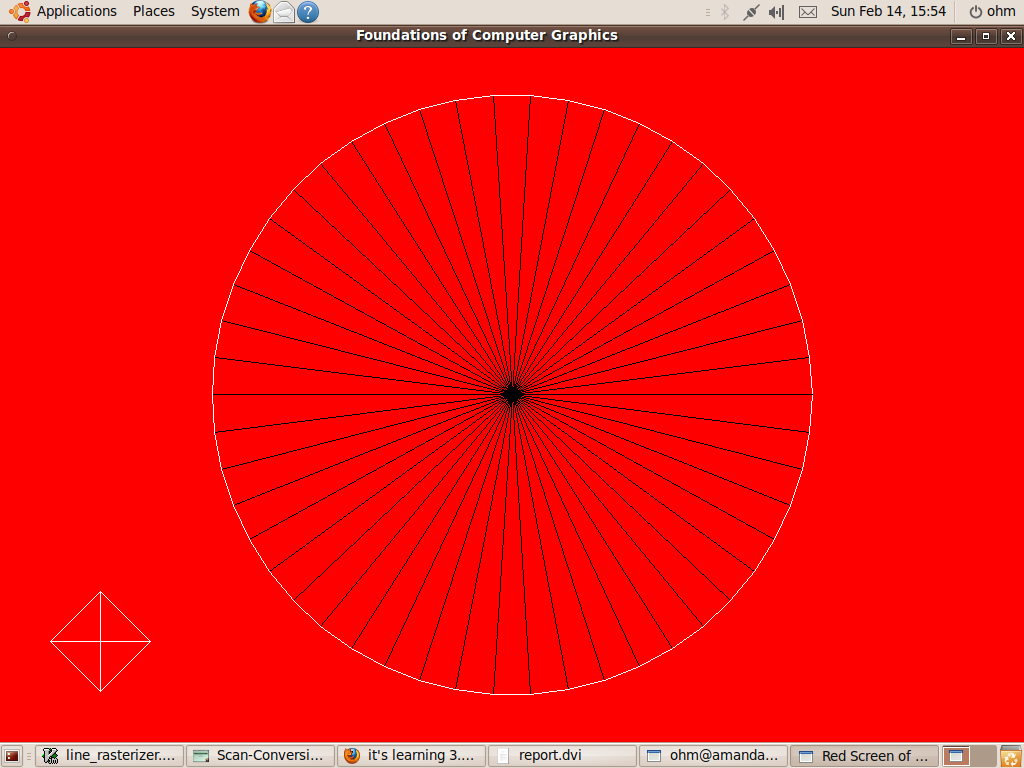
\includegraphics[width=0.99\textwidth]{lines.eps}
\end{center}

\begin{center}
\centering
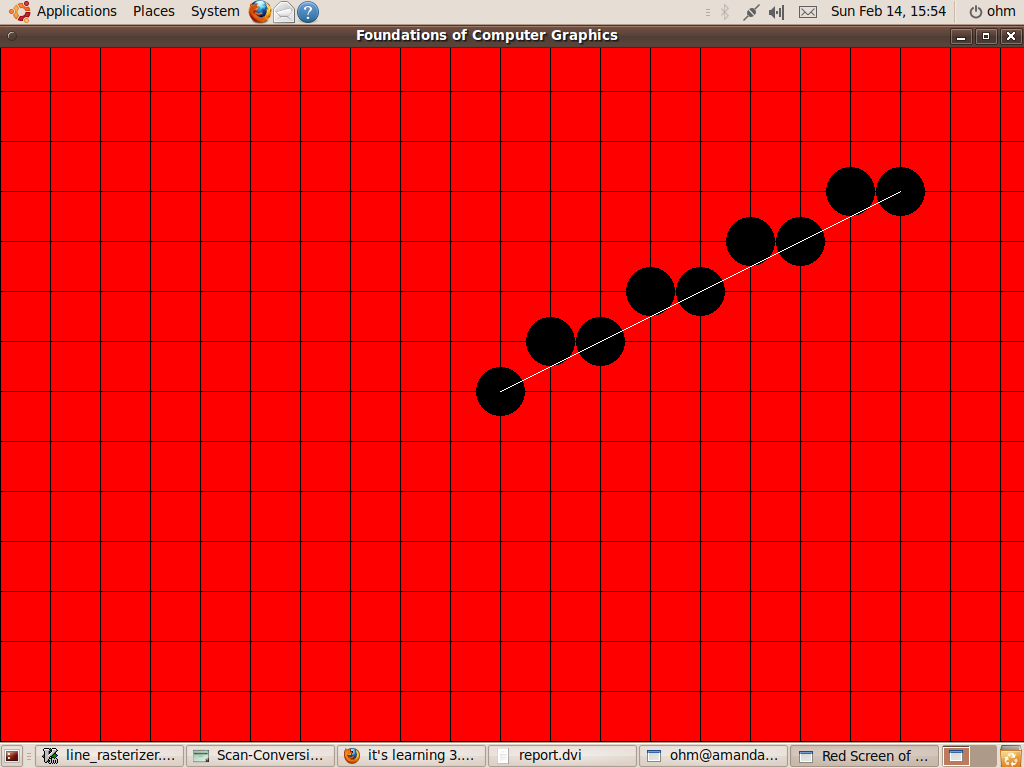
\includegraphics[width=0.99\textwidth]{debuglines.eps}
\end{center}

Da det er svært at se hvad der sker på disse to billeder, har jeg også vedlagt dem min rapport i størrelse 1024 gange 768.
Dette er slutningen på ugeopgave 2.


\end{document}
